% Time-stamp: <2025-02-26 18:15:25>


\documentclass[presentation,aspectratio=1610]{beamer}

%% Full theme: AnnArbor Antibes Bergen Berkeley Berlin Boadilla boxes CambridgeUS Copenhagen Darmstadt default Dresden EastLansing Frankfurt Goettingen Hannover Ilmenau JuanLesPins Luebeck Madrid Malmoe Marburg Montpellier PaloAlto Pittsburgh Rochester Singapore Szeged Warsaw
% \usetheme{Luebeck}

%% outer themes (header/footer): default infolines miniframes smoothbars sidebar split shadow tree smoothtree
% \useoutertheme[subsection=false]{smoothbars}
% \usetheme{Rochester}
 \useoutertheme{split}

%% inner theme (content): default circles rectangles rounded inmargin
\useinnertheme{rectangles}

\usecolortheme{beaver}

\input{style}



\defcolvar{n}{n}{red}
\defcolvar{l}{\ell}{blue}

\title{Symmetric Techniques for Advanced Protocols: What *are* They?}
\author[Léo Perrin]{Léo Perrin\inst{1} }

\institute{Inria, Paris}
\titlegraphic{\includegraphics[height=1.1cm]{figures/inria}}


\date{14th of March 2025}




\begin{document}

{
  \pagestyle{empty}

  \maketitle


  \begin{frame}{Trendy topics}

    \begin{itemize}
      \large
    \item [] MPC-friendly? 
    \item [] Arithmetization-Oriented?
    \item [] Verification efficiency?
    \item [] Algebraic attacks? \pause
    \item [] Symmetric crypto \textbf{for the blockchain...} \pause
    \item [] \alert{... for neural networks???}
    \end{itemize}
    \begin{center}
      The conclusion of today: \textbf{symmetric cryptography} has always had to deal with specific \textbf{implementation criteria}, but the \alert{new ones} are indeed a bit \textbf{stranger than before}.
    \end{center}
  \end{frame}
}


\tocStartsAppearingHere{}


\section{What is the Purpose of a Symmetric Primitive}

\subsection{Let's look at primitives we all know}


\begin{frame}{Let's talk!}
  \vfill

  \begin{center}
    \includegraphics[width=8cm]{./figures/simpsons}
  \end{center}
  
  \vfill
\end{frame}


\begin{frame}{Unstable Definitions}
  \begin{alertblock}{What is ``efficient'' varies}
    \begin{itemize}
    \item What are the operations that we \textbf{can} use?
    \item What are the associated \textbf{costs}? 
    \end{itemize}
    \begin{center}
      How to get the best security for a given price?
    \end{center}
  \end{alertblock}

  
  
  \begin{exampleblock}{What is ``secure'' varies}
    \begin{itemize}
    \item Should the primitive work in many context? \hfill\onslide<4>{Modularity vs. Single use}
    \item Do we care about nonce-misuse? \hfill\onslide<4>{Robustness vs. ``not our problem''}
    \item
    \end{itemize}
    \begin{center}
      How do we define the security that the primitive must provide?
    \end{center}
  \end{exampleblock}
\end{frame}


\subsection{A Small Cog in a Big Machine}


\begin{frame}{Web Encryption}
  \begin{center}
    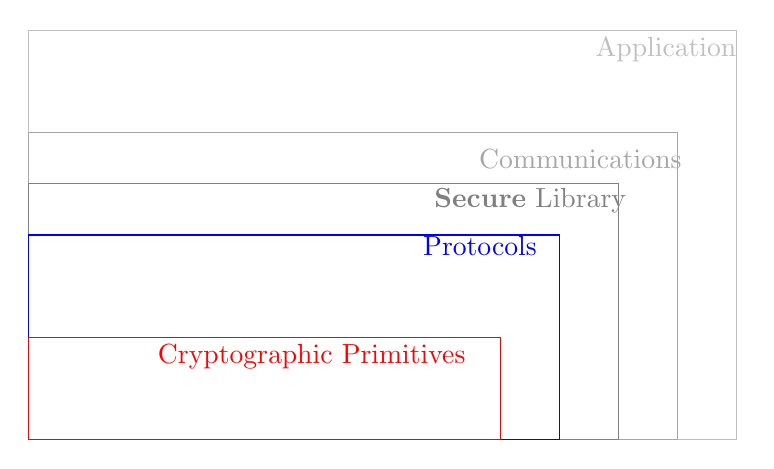
\begin{tikzpicture}[xscale=1.5,yscale=1.3]
      \draw[color=gray!50!white] (0, 0) rectangle (6, 4) node[pos=0.9,above] {Application};
      \onslide<2->{
        \draw[color=gray!70!white] (0, 0) rectangle (5.5, 3) node[pos=0.85,above] {Communications};
      }
      \onslide<3->{
        \draw[color=gray] (0, 0) rectangle (5, 2.5) node[pos=0.85,above] {\textbf{Secure} Library};
      }
      \onslide<4->{
        \draw[color=blue] (0, 0) rectangle (4.5, 2) node[pos=0.85,above] {Protocols};
      }
      \onslide<5->{
        \draw[color=red] (0, 0) rectangle (4, 1) node[pos=0.6,above] {Cryptographic Primitives};
      }
    \end{tikzpicture}

    \begin{itemize}
    \item<6-> We want \alert{software efficient} (computer and smartphone but not micro-controllers) efficient \alert{AEAD}.
    \item<7> AES-GCM; Chacha-poly1305.
    \end{itemize}
  \end{center}
\end{frame}



\begin{frame}{RAM Encryption}
  \begin{center}
    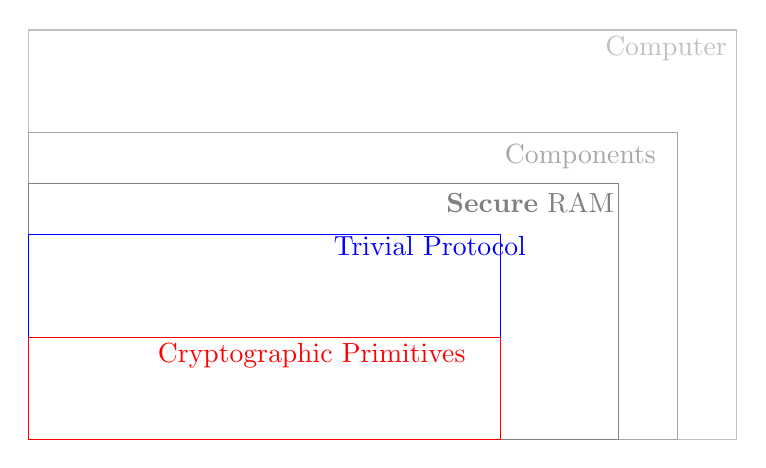
\begin{tikzpicture}[xscale=1.5,yscale=1.3]
      \draw[color=gray!50!white] (0, 0) rectangle (6, 4) node[pos=0.9,above] {Computer};
      \onslide<2->{
        \draw[color=gray!70!white] (0, 0) rectangle (5.5, 3) node[pos=0.85,above] {Components};
      }
      \onslide<3->{
        \draw[color=gray] (0, 0) rectangle (5, 2.5) node[pos=0.85,above] {\textbf{Secure} RAM};
      }
      \onslide<4->{
        \draw[color=blue] (0, 0) rectangle (4, 2) node[pos=0.85,above] {Trivial Protocol};
      }
      \onslide<5->{
        \draw[color=red] (0, 0) rectangle (4, 1) node[pos=0.6,above] {Cryptographic Primitives};
      }
    \end{tikzpicture}

    \begin{itemize}
    \item<6-> We want \alert{very low latency} \alert{block encryption}.
    \item<7> PRINCE? QARMA? not so clear at this stage.
    \end{itemize}
  \end{center}
\end{frame}


\begin{frame}{Some Constants}
  \begin{itemize}
    \setlength\itemsep{1cm}
    \large
  \item A symmetric primitive is very \alert{small} (but crucial) cog in a
    very big machine, \pause
  \item there are many \alert{different} ``big machines'', and \pause
  \item this has a \alert{huge influence} on what the primitive looks like.
  \end{itemize}
\end{frame}


\section{New Protocols}


\section{Conclusion}

\begin{frame}{Conclusion}
  \pause\vspace{1cm}
  
  \begin{center}
    \textbf{Thank you!}
  \end{center}
\end{frame}

\end{document}


% Local Variables:
% compile-command: "xelatex presentation.tex"
% End:
